\notechapter{N-20251114}{Teichmueller Theory Without One Universe: Classical Deformation, Hodge Theaters, and Identification}

\section{Why the word Teichmueller matters}

The word ``Teichmueller'' in inter-universal Teichmueller theory should not be treated as a poetic label.  It points to a deformation problem.  In classical Teichmueller theory, one fixes a topological surface and studies how complex structures on that surface vary.  In IUT, the analogy is not that arithmetic curves literally form a classical Teichmueller space.  The analogy is that some structures are treated as rigid reference data, while other structures are deformed and measured.

This note compares the two situations.  The comparison is useful only if it is kept precise.  Classical Teichmueller theory varies complex structures inside a common topological background.  IUT tries to compare arithmetic data across distinct theaters where ordinary ring-theoretic identification is not allowed.  The controversial strength of the theory is already visible at this level: it replaces the ordinary demand for one common universe by a system of reconstructed, multiradial, and indeterminacy-controlled comparisons.

\section{Classical Teichmueller theory: fixed topology, variable complex structure}

Let \(S\) be an oriented topological surface of finite type.  To remember which complex surface is supposed to be a deformation of \(S\), one uses a marking.

\begin{definition}[Marked Riemann surface]
A marked Riemann surface modeled on \(S\) is a pair
\[
  (X,f),
\]
where \(X\) is a Riemann surface and
\[
  f:S\longrightarrow X
\]
is an orientation-preserving homeomorphism, or more generally a quasiconformal map, regarded up to homotopy.
\end{definition}

The marking is the key device.  Without it, one has only a collection of complex curves.  With it, different complex structures can still be compared as structures on the same underlying topological surface.

\begin{definition}[Teichmueller space]
The Teichmueller space \(T(S)\) is the set of equivalence classes of marked Riemann surfaces \((X,f)\), where
\[
  (X,f)\sim(Y,g)
\]
if there is a biholomorphism \(h:X\to Y\) such that \(h\circ f\) is homotopic to \(g\).
\end{definition}

Thus classical Teichmueller theory separates two layers:
\[
  \text{topological surface } S
  \qquad\text{and}\qquad
  \text{complex structure on } S.
\]
The topology is the reference frame.  The complex structure is what moves.

\begin{remark}[The role of marking]
A marking is an authorized identification.  It tells us when two points of Teichmueller space represent two complex structures on the same underlying surface.  This will be the main contrast with IUT: IUT cannot simply use a single marking to identify all ring structures across its theaters.
\end{remark}

\section{Distortion is measured in one universe}

Teichmueller theory does not only parametrize complex structures.  It measures deformation by quasiconformal distortion.

\begin{definition}[Quasiconformal distortion]
Let \(f:X\to Y\) be a quasiconformal map between Riemann surfaces.  In a local coordinate it has distributional derivatives \(f_z\) and \(f_{\bar z}\).  Its Beltrami coefficient is
\[
  \mu_f=\frac{f_{\bar z}}{f_z},
\]
and the maximal dilatation is
\[
  K(f)=\frac{1+\|\mu_f\|_{\infty}}{1-\|\mu_f\|_{\infty}}.
\]
\end{definition}

The Teichmueller distance is then defined by minimizing distortion among maps in the correct homotopy class:
\[
  d_T((X,f),(Y,g))
  =\frac12\inf_h \log K(h),
\]
where \(h:X\to Y\) ranges over quasiconformal maps such that \(h\circ f\) is homotopic to \(g\).

The important point is structural: this distance makes sense because the comparison is made inside one clear framework.  Both surfaces are marked by the same \(S\).  The phrase ``same underlying topological surface'' has a precise meaning.

\begin{proposition}[Classical deformation has a common reference object]
In classical Teichmueller theory, the comparison of two complex structures is mediated by the fixed surface \(S\).  The marking supplies a legitimate way to say that the two complex structures are structures on the same object.
\end{proposition}

\begin{proof}
A point of \(T(S)\) is not merely a Riemann surface \(X\); it is a pair \((X,f)\).  Given two points \((X,f)\) and \((Y,g)\), the maps \(f\) and \(g\) identify both surfaces with the same topological source \(S\), up to homotopy.  Therefore quasiconformal maps \(h:X\to Y\) can be tested against the homotopy condition \(h\circ f\simeq g\).  The fixed \(S\) is the common reference object.
\end{proof}

\section{Why the arithmetic analogy cannot be literal}

In the arithmetic setting, the objects are not Riemann surfaces equipped with varying complex structures.  The basic geometric objects are hyperbolic curves, elliptic curves with punctures or orbifold quotients, number fields, local fields, arithmetic fundamental groups, and Galois groups.  The rigid structure is no longer a topological surface.  It is closer to a package of fundamental-group-like data from which ring structures can be reconstructed.

\begin{definition}[Arithmetic fundamental-group reference data, schematic]
For a hyperbolic curve \(X\) over a number field \(K\), the arithmetic fundamental group fits into an exact sequence
\[
  1\longrightarrow \pi_1^{\mathrm{geom}}(X)
  \longrightarrow \pi_1(X)
  \longrightarrow G_K
  \longrightarrow 1.
\]
In the IUT entrance, such group-theoretic data acts as a rigid reference structure from which arithmetic and ring-theoretic data may be reconstructed by mono-anabelian methods.
\end{definition}

The analogy with classical Teichmueller theory is therefore shifted:
\[
\begin{array}{ccl}
\text{classical theory} &:&
\text{fixed topological type, variable complex structure},\\[2mm]
\text{IUT direction} &:&
\text{rigid group-theoretic data, deformed ring-theoretic presentations}.
\end{array}
\]
This is only an analogy, but it is a mathematically meaningful one.

\begin{remark}[What should not be inferred]
The word ``Teichmueller'' does not mean that IUT constructs a Teichmueller space of number fields in the classical sense.  It means that the theory is organized around deformation, rigidity, and comparison of structures, but the structures being compared are arithmetic and group-theoretic rather than complex-analytic.
\end{remark}

\section{Hodge theaters as arithmetic stages}

The language of theaters is one of the points where IUT becomes unfamiliar.  A theater should not be imagined as a parallel universe in a science-fiction sense.  It is a package of data within which certain arithmetic, geometric, and group-theoretic structures can be discussed internally.

\begin{definition}[Hodge theater, working schematic]
In this note, a Hodge theater means a package of arithmetic data containing several mutually related layers: local fields, number-field data, arithmetic fundamental groups, monoid-theoretic data, and theta-data.  The full definition in IUT is much more elaborate.  The working point is that a theater provides an internal stage on which ring structures, Galois data, theta-values, and reconstruction algorithms coexist.
\end{definition}

The word ``theater'' is useful because IUT does not simply compare two rings by a ring isomorphism.  It compares data internal to one theater with data internal to another theater through special links.

\begin{definition}[Inter-universal comparison, schematic]
An inter-universal comparison is a comparison between data belonging to distinct Hodge theaters, where one does not assume a global ring-theoretic identification between the theaters.  The comparison is mediated by structures such as theta-links, log-links, Kummer correspondences, and mono-anabelian reconstruction.
\end{definition}

In ordinary algebraic geometry, the most comfortable comparison has the form
\[
  R\cong R'
\]
or at least a morphism of schemes.  In IUT, the central horizontal comparison is not of that kind.  The theta-link is precisely a link that deforms ring-theoretic structure rather than preserving it.

\section{Etale-like and Frobenius-like directions}

Fesenko's survey uses the distinction between structures that behave like rigid etale or fundamental-group data and structures that behave more like monoid-theoretic or Frobenius-type data.  This is one of the cleanest ways to understand why ordinary scheme morphisms are not enough.

\begin{definition}[Etale-like and Frobenius-like structures, schematic]
An etale-like structure is a structure on the fundamental-group side: it is functorial, rigid, and invariant enough to be used for reconstruction.  A Frobenius-like structure is a monoid-theoretic structure used to build deformation links, especially when no ordinary Frobenius morphism of number fields exists.
\end{definition}

The terminology is suggestive.  Over a field of positive characteristic, the Frobenius map \(x\mapsto x^p\) is a genuine morphism.  For number fields, there is no such global Frobenius endomorphism.  IUT instead builds categorical and monoid-theoretic analogues that can play a deformation role.

\begin{remark}[The arithmetic reason this is radical]
The theory tries to get a Frobenius-like deformation effect in a setting where the usual Frobenius morphism does not exist.  This is part of the reason the comparison cannot remain inside ordinary scheme-theoretic geometry.
\end{remark}

\section{The theta-link is the point where one universe breaks}

The local model already appeared in the previous two notes:
\[
  q_v\longmapsto q_v^{m^2},
  \qquad
  u\longmapsto u.
\]
This operation is meaningful on the multiplicative/monoid side, but it is not a ring homomorphism.  It therefore cannot serve as an identification of local fields as rings.

\begin{proposition}[No common ring is carried by the theta-link]
If a theta-link is interpreted as the assignment that carries a Tate parameter \(q\) to theta-values behaving like \(q^{m^2}\) while keeping unit data on the monoid side, then it cannot be regarded as a ring-theoretic isomorphism between the source and target local structures.
\end{proposition}

\begin{proof}
A ring-theoretic isomorphism must preserve addition and multiplication simultaneously.  The theta-link is constructed from multiplicative monoids, unit groups, Tate parameters, and theta-values.  Its displayed local behavior is not an additive operation.  Therefore treating it as a ring isomorphism would add a compatibility that the construction is not designed to provide.
\end{proof}

This is the exact mathematical sense in which the ``one universe'' picture breaks.  If one tries to force the two sides of the theta-link into the same ring-theoretic universe, one loses the deformation that the theta-link was built to express.

\section{The log-link does not restore naive equality}

The log-link exists because the theta-link moves multiplicative data while the final Diophantine inequality needs additive and volume information.  The nonarchimedean logarithm
\[
  \log:\mathcal O_L^{\times}\longrightarrow L
\]
translates unit data into additive data.  This does not mean that the original ring structure has been transported unchanged.

\begin{definition}[Recovered additive data, schematic]
Recovered additive data means additive structure obtained after applying logarithmic and mono-anabelian reconstruction procedures to multiplicative or group-theoretic data.  It is not the same thing as an additive structure transported by a ring isomorphism.
\end{definition}

The distinction is small in words but large in mathematics.  Classical Teichmueller theory deforms complex structures while markings keep track of the same underlying topological surface.  IUT deforms arithmetic structures in a way that prevents one from identifying the two sides as the same ring.  Additive information must therefore be reconstructed rather than simply carried over.

\begin{remark}[Why the log-shell is needed]
The log-link and the theta-link do not give a clean commutative square of elementwise identifications.  The log-shell provides a controlled container for the resulting ambiguity.  It is a way of replacing exact equality by a bounded or contained region in which the relevant images live.
\end{remark}

\section{Classical marking versus multiradial reconstruction}

The most useful comparison between classical Teichmueller theory and IUT is not a slogan about deformation.  It is a comparison between two ways of controlling identity.

The comparison can be kept in five pairs.
\begin{enumerate}
  \item Classical theory chooses a fixed topological surface \(S\); IUT treats arithmetic fundamental-group-like data as rigid and reconstructive.
  \item Classical theory uses a marking \(f:S\to X\); IUT uses mono-anabelian algorithms to recover ring-theoretic data from group-theoretic input.
  \item Classical theory moves the complex structure on \(S\); IUT moves a ring-theoretic or monoid-theoretic presentation of arithmetic data.
  \item Classical theory measures distortion by quasiconformal maps; IUT creates and measures arithmetic deformation by theta-links and log-links.
  \item Classical comparison remains inside one marked topological setting; IUT comparison moves across distinct Hodge theaters.
\end{enumerate}

This list shows why IUT is not merely difficult notation.  The role played by marking in classical Teichmueller theory is not replaced by one simple arithmetic marking.  Instead, it is replaced by a much more elaborate system: reconstruction algorithms, label symmetries, Kummer theory, log-shells, and indeterminacies.

\begin{definition}[Multiradial identification, schematic]
A multiradial identification is not a direct equality of objects in one common ring universe.  It is an identification of reconstructed structures that remains meaningful when viewed from several theaters or spokes at once.
\end{definition}

This is why multiradiality is conceptually central.  If a construction only makes sense from one spoke, it may depend on a hidden choice of coordinates.  A multiradial construction is designed to survive the change of theater.

\section{The mathematical source of the controversy}

This note should not become a news summary.  The mathematical tension can be stated without naming any episode.  It is a tension about legitimate identification.

\begin{proposition}[The identification burden]
Once ordinary ring-theoretic identification is forbidden across theaters, every later comparison must justify itself by some replacement mechanism: mono-anabelian reconstruction, Kummer correspondence, theta-link compatibility, log-link compatibility, multiradiality, or a controlled indeterminacy.
\end{proposition}

\begin{proof}
Without a ring isomorphism, there is no default rule saying that an element, sum, unit, valuation, or theta-value in one theater is the same object as an element, sum, unit, valuation, or theta-value in another.  Therefore each permitted comparison must be constructed and checked.  The structures listed in the statement are precisely the devices introduced to make such comparisons possible without collapsing all theaters into one ordinary ring-theoretic setting.
\end{proof}

The controversial foundational move is therefore not merely ``there are many universes''.  A vague multiverse would have no mathematical force.  The real move is this: do not identify rings directly; instead recover and compare selected structures by controlled algorithms.  The difficulty is that the replacement mechanisms must be strong enough to support the final log-volume inequality.  If they are too weak, the deformation cannot be measured.  If they are interpreted as ordinary equalities, the deformation disappears.

\begin{remark}[Why a one-universe reading is dangerous]
A one-universe reading tries to place all theaters into a single background in which ordinary ring-theoretic equality is available.  That may make the theory look more familiar, but it changes the object under study.  The theta-link is designed precisely to avoid being a ring-theoretic identification.
\end{remark}

\section{A compact model of the logic}

The logical structure of the comparison can be summarized as follows:
\begin{center}
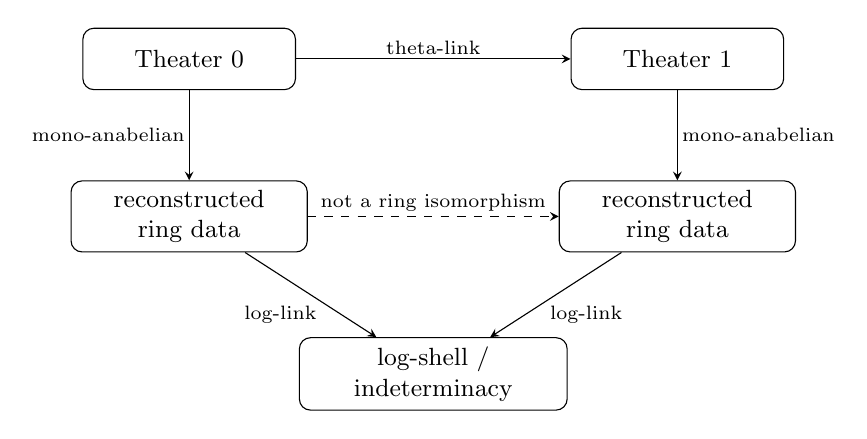
\begin{tikzpicture}[
  >=stealth,
  nodebox/.style={draw,rounded corners,align=center,minimum height=0.78cm,font=\small},
  edgelabel/.style={fill=white,inner sep=1.5pt,font=\scriptsize}
]
  \node[nodebox,minimum width=2.7cm] (T0) at (-3.1,0) {Theater \(0\)};
  \node[nodebox,minimum width=2.7cm] (T1) at ( 3.1,0) {Theater \(1\)};
  \node[nodebox,minimum width=3.0cm] (R0) at (-3.1,-2.0) {reconstructed\\ring data};
  \node[nodebox,minimum width=3.0cm] (R1) at ( 3.1,-2.0) {reconstructed\\ring data};
  \node[nodebox,minimum width=3.4cm] (S)  at ( 0,-4.0) {log-shell /\\indeterminacy};

  \draw[->] (T0) -- node[edgelabel,above] {theta-link} (T1);
  \draw[->] (T0) -- node[edgelabel,left] {mono-anabelian} (R0);
  \draw[->] (T1) -- node[edgelabel,right] {mono-anabelian} (R1);
  \draw[->] (R0) -- node[edgelabel,below left,pos=0.58] {log-link} (S);
  \draw[->] (R1) -- node[edgelabel,below right,pos=0.58] {log-link} (S);
  \draw[dashed,->] (R0) -- node[edgelabel,above] {not a ring isomorphism} (R1);
\end{tikzpicture}
\end{center}
The dashed arrow is the temptation that the theory resists.  The comparison does not proceed by declaring the two reconstructed rings equal.  It proceeds by controlling how their relevant images sit inside the logarithmic and theta-theoretic structures.

\section{What this third note establishes}

The relationship with classical Teichmueller theory can now be stated cleanly.

\begin{enumerate}
  \item Classical Teichmueller theory fixes a topological surface and deforms complex structures on it.
  \item The marking is the mechanism that makes comparison legitimate in the classical theory.
  \item IUT does not have a single arithmetic marking that identifies all ring structures across theaters.
  \item Instead, IUT uses Hodge theaters, theta-links, log-links, mono-anabelian reconstruction, Kummer theory, multiradiality, and indeterminacies.
  \item The phrase ``inter-universal'' means that comparisons are made without collapsing the theaters into one ordinary ring-theoretic universe.
  \item The deepest mathematical pressure point is therefore the legitimacy and strength of these replacement identifications.
\end{enumerate}

The theory is difficult not only because it contains many objects, but because it changes the usual rule of comparison.  Classical Teichmueller theory asks how complex structures vary when the underlying topological object is held fixed.  IUT asks how arithmetic structures can be deformed when the ordinary ring structure is not allowed to serve as a common background.  That is the mathematical content behind the word ``inter-universal''.
